\chapter{Konzeption}
\label{chapter-konzept}

In diesem Kapitel wird die eigentliche Erkenntnis der Arbeit beschrieben. Die
eingangs beschreibenen Anforderungen definieren was das System zu leisten hat.
Im folgenden werden die Funktionalitäten definiert, um zu beschreiben, wie das
System die Anforderungen gewährleisten kann. Desweiteren wird auf die Wahl der
Frameworks und darausfolgend auf die Systemarchitektur eingeggangen.

\section{Funktionalität}
\label{section:funktionalitaeten}
Im folgenden werden die für das System relevanten Funktionalitäten aufgeführt.
ZUr besseren Lesbakeit wurden die Funktionalitäten nach Benutzergruppen
aufgeteilt.

% Funktionalitäten für Verleihende und Ausleihende
\subsection{Funktionalitäten für Verleihende und Ausleihende}
Im Folgenden werden Funktionalitäten, welche für Verleihende und Ausleihenden
von Bedeutung sind näher erläutert (\ref{table:ft-va}).

\begin{table}[h]
    \centering
    \caption{Funktionalitäten für Verleihende und Ausleihende}
    \begin{longtable}{lll}
        \arrayrulecolor{maincolor}\hline
        \sffamily\color{maincolor}ID & \sffamily\color{maincolor}Titel        &
        \sffamily\color{maincolor}Anforderungen
        \\
        \arrayrulecolor{maincolor}\hline
        Ft-VA-1                      & Übersicht über ausleihbare Assets      &
        \anfref{V20} \anfref{Z20} \anfref{F50} \anfref{K10} \anfref{F10}
        \anfref{F30}                                                            \\
        Ft-VA-2                      & Benachrichtigungen \& Erinnerungen     &
        \anfref{F100} \anfref{F110} \anfref{F120}                               \\
        Ft-VA-3                      & Sichtbarkeit von Ansprechpartner:innen &
        \anfref{F50}                                                            \\
        Ft-VA-4                      & Authentifizierung per IDM Account      &
        \anfref{F70} \anfref{F80}                                               \\
        \arrayrulecolor{maincolor}\hline
    \end{longtable}
    \label{table:ft-va}
\end{table}

{\sffamily\color{maincolor}{Ft-VA-1 | Übersicht über ausleihbare Assets }}\\
Die Übersicht, der am IMIS vorhandenen Assets, wurde mittels Kategorien
umgesetzt. Dazu gibt es eine Übersicht, bei der alle Assets eingesehen werden
können. Die einzelnen Kategorien beeinhalten Unterkategorien. In der Übersicht
werden Informationen, wie Name, Seriennummer, Marke und Status eines Assets
angezeigt. Wie bereits in der Problemanalyse geschildet
(\ref{section:probleme-allgemein}) gibt es keine Übersicht, über ausleihbare
Assets. Dies zeigt die Dringlichkeit des SnipeIT Companion für eine besser
Vorbereitung.

    {\sffamily\color{maincolor}{Ft-VA-2 | Benachrichtigungen \& Erinnerungen
        }}\\
Verleihende werden nach dem Abschluss eines von ihnen verantwortlichen Assets
benachrichtigt. Die Benachrichtigung umfasst Informationen, wer das Asset, wann
rserviert hat, und wann die Abholung für das Assets stattfinden soll. Außerdem
wird es eine direkte weiterleitungs möglichkeit geben, sollten Verleihenden nich
können. Deweiterne Erhalten Ausleihende Erinnerungen, sobald die Abholung und
Rückgabe eines Assets ansteht.

    {\sffamily\color{maincolor}{Ft-VA-3 | Sichtbarkeit von
            Ansprechpartner:innen}}\\
Für Rückfragen zu einem Asset sind Kontaktinformation zu Ansprechpartner:innen
(Verleihende) sowie deren E-Mail-Adresse direkt ersichtlich.

Nachdem der Checkout stattgefunden hat, erhalten Verleihende eine
Zusammenfassung über die Ausleihdaten und eine  Hinweis, wann die Abholung
stattfindet. Außerdem werden Kontaktinformation des Verleihenden angezeigt
(Name, E-Mail und Lageort des Assets).


    {\sffamily\color{maincolor}{Ft-VA-4 | Authentifizierung per IDM Account}}\\
Mit hilfe einer Verknüpfung über den LDAP Account der Universität zu Lübeck,
können sich Nutzende mit ihrem bereits existierenden IDM Account einloggen, so
muss kein Neues Konto erstellt werden und die Zuständigkeit, sowie sicherheit,
wer sich einloggt ist gegeben.

\subsection{Funktionalitäten für Verleihende}
Im Folgenden werden Funktionalitäten, welche für Verleihende von Bedeutung sind
näher erläutert (\ref{table:ft-v}).

\begin{table}[h]
    \centering
    \caption{Funktionalitäten für (V)erleihenden}
    \begin{longtable}{lll}
        \arrayrulecolor{maincolor}\hline
        \sffamily\color{maincolor}ID & \sffamily\color{maincolor}Titel &
        \sffamily\color{maincolor}Anforderungen
        \\
        \arrayrulecolor{maincolor}\hline
        Ft-V-1                       & Verfügbarkeit von Assets        &
        \anfref{V20} \anfref{Z20} \anfref{F50} \anfref{K10} \anfref{F10}
        \anfref{F30}                                                     \\
        Ft-V-2                       & Zuständigkeitsbereich           &
        \anfref{F50}                                                     \\
        Ft-V-3                       & Bearbeiten des Assetstatus      &
        \anfref{F150}                                                    \\
        Ft-V-4                       & Pflege von Assets               &
        \anfref{F130}                                                    \\
        Ft-V-5                       & Pflege der Datenbank            &
        \anfref{F140}                                                    \\
        \arrayrulecolor{maincolor}\hline
    \end{longtable}
    \label{table:ft-v}
\end{table}

{\sffamily\color{maincolor}{Ft-V-1 |  Verfügbarkeit von Assets }}\\
Verleihende benötigen einen Überblick, über den Status der Assets. Dies wird
untereinandem durch einen Kalender mit Filter- und Suchfunktion ermöglicht.

{\sffamily\color{maincolor}{Ft-V-2 | Zuständigkeitsbereich }}\\
Um für Ausleihende Kontaktinformationen anzeigen zu können \textit{(Ft-A-6)},
müssen die Zuständigkeitsbereich eingetragen werden können. Außerdem sollten
alternative Ansprechpartner:innen kenntlich gemacht werden, um Abholtermine
aufgrund von Krankheit oder Homeoffice nicht verschieben zu müssen.


{\sffamily\color{maincolor}{Ft-V-3 | Bearbeiten des Assetstatus }}\\
Assets, welche an Ausleihende übergeben wurde, müssen zunächst manuell in ihrem
Status bestätigt werden. Hierfür ist eine simple Funktion vorgesehen, sodass der
Status des Assets schnell aktuell gehalten werden kann. Außerdem soll das
System, nachdem eine Abholung oder Rückgabe stattgefunden hat, eine
Benachrichtigung an Verleihende senden, sollte der Status nicht bereits
bestätigt worden sein.

    {\sffamily\color{maincolor}{Ft-V-4 | Pflege von Assets   }}\\
Mit Hilfe der Zuständigkeitsbereich \textit{(Ft-V-2)} kann die Pflege der Assets
besser kontrolliert werden. Außerdem können durch Erinnerungen und Checkliste
Wartungen weniger leicht vergessen werden und besser aufgeteilt werden.

    {\sffamily\color{maincolor}{Ft-V-5 | Pflege der Datenbank }}\\
DAs Prinzip des Reservierungstools kann nur funktionieren, wenn Neuanschaffung
in die Datenbank eingepflegt werden. Hierfür soll eine Anleitung für Verleihende
sichtbar gemacht werden. Wichtig hierbei ist, dass das Einpflgen nicht nur für
das Ausleihen hilfreich ist, sondern auch für eine generelle Übersicht des
bestands am \ac{imis}.



\subsection{Funktionalitäten für Ausleihende}
Im Folgenden werden Funktionalitäten, welche für Ausleihenden von Bedeutung sind
näher erläutert (\ref{table:ft-A}).


\begin{table}[h]
    \centering
    \caption{Funktionalitäten für (A)usleihenden}
    \begin{longtable}{lll}
        \arrayrulecolor{maincolor}\hline
        \sffamily\color{maincolor}ID & \sffamily\color{maincolor}Titel &
        \sffamily\color{maincolor}Anforderungen
        \\
        \arrayrulecolor{maincolor}\hline
        Ft-A-1                       & Material-Suche                  &
        \anfref{V20} \anfref{Z20} \anfref{K10} \anfref{F10} \anfref{F30}
        \\
        Ft-A-2                       & Filtern und Sortieren           &
        \anfref{V30} \anfref{F30} \anfref{F70}                               \\
        Ft-A-3                       & Ausleihhilfe                    &
        \anfref{V30}\anfref{F70}                                             \\
        Ft-A-4                       & Startseite                      &
        \anfref{F60}                                                         \\
        Ft-A-5                       & Reservierungs-Checkout          &
        \anfref{F60} \anfref{F150}                                           \\
        Ft-A-6                       & Detailansicht                   &
        \anfref{V50} \anfref{Z30} \anfref{F40} \anfref{F50}                  \\
        Ft-A-7                       & Rückgabe-Checkliste             & ???
        \\
        \arrayrulecolor{maincolor}\hline
    \end{longtable}
    \label{table:ft-A}
\end{table}

{\sffamily\color{maincolor}{Ft-A-1 | Material-Suche }}\\
Die Material-Suche dient zum einen einer simplen aber unterstütztende
Kategorieneinteilung, zum anderen für das gezielte Suchen nach Verfügbarkeiten
(verfügbar, Nicht verfügbar und Hinweis). Das gezielte Suchen nach Verfügbarkeit
wird durch die AUfforderung den Ausleihzeitraum auszuwählen ermöglicht.
Daraufhin gibt es die Möglichkeit gewünschtest Material in einem Suchfeld
einzugeben oder über die Kategorien nach dem Asset zu suchen. Das Suchenfeld
gibt bereits beim eintippen Vorschläge. Die Vorschläge können das Assets direkt,
die Kategorie oder ... sein. Bei mehreren Assets gibt die Suche mithilfe einer
Aufzählung alle Elemente an, die bereits afür die Reservierung ausgewählt
wurden.

    {\sffamily\color{maincolor}{Ft-A-2 | Filtern und Sortieren }}\\
Um das Finden für Assets leichter zu gestalten sollen Nutzende sets nach
Kategorie, Nutzen und Verfügbarkeit filtern können. Außerdem ist das sortieren
von A-Z oder Z-A, sowie nach den Verfügbarkeiten möglich.

{\sffamily\color{maincolor}{Ft-A-3 | Ausleihhilfe  }}\\
Die Ausleihhilfe ist eine vereinfachte Form eines Assistenten. Die Suche nach
Nutzen, wie Videodreh mit Ton und draußen, soll dem Nutzenden Vorschläge geben
können. Dies soll insbesondere Ausleihende unterscützen, die in den bereichen
noch nicht viel Expertise mitbringen können. Außerdem soll es Verleihenden den
Ausleihprozess erleichtern, weil das Beratunggespräch (Aufgabe Ref) wegfallen
kann.

    {\sffamily\color{maincolor}{Ft-A-4 | Startseite }}\\
Die Startseite soll nutzenden helfen, eine  Überblick zu erlangen. Für
erstnutzende, sind hinweise für die Materal-Suche und Ausleihhilfe in Form von
Button gegebn. Für Nutzende, die bereits etwas ausgeliehen haben, wird eine
Übersicht über Ausleihe und vergangenes Material angezeigt. wichtige
Informationen, wie der Zeitraum werden direkt auf einen Blick ersichtlich.

    {\sffamily\color{maincolor}{Ft-A-5 | Reservierungs-Checkout }}\\
Mit Hilfe des Reservierungs-Checkouts können alle ausgewählten Assets im
Überblick eingesehen werdenn. Außerdem werden alle Ausleihdaten, wie Zeitraum
der Ausleihe, Abholung und Rückgabe aufgeführt. Desweiteren sollte es die
Möglichkeit, alle Ausleihdaten bearbeiten zu können, sollte ein Datum oder eine
Uhrzeit nicht passen. Abschließend werden die Regeln und SIcherheitshinwweise
aufgeführt. Mithilfe einer AGB Bla erklärung, gilt die Materialausleihe als
vertraglich abgeschlossen.

    {\sffamily\color{maincolor}{Ft-A-6 | Detailsansicht }}\\
In der Detailansicht werden die Assets und deren Eigenschaften dargestellt.
Hierbei werden Informationen wie: Name, Seriennummer, Artikelbeschreibung,
Technischedetaisl, Kontaktinformation der Verleihenden, ... dargestellt.
Außerdem wird hier die Möglichkeit gegebn, Den Ausleihzeitraum einzustellen und
einzusehen, wann ein Asset verfügbar ist. In Form eines Button wird sichtbar,
dass das Asset zur Ausleihe hinzugefügt werden kann.

    {\sffamily\color{maincolor}{Ft-A-7 | Rückgabe-Checkliste}}\\
Bevor die ausgeliehenen Assets an Verlehende zurückgeben werden, wird eine
Checkliste für das jeweilige Asset angezeigt, bei der Hinweise stehen wie:
SD-Karte geleert, Assets auf Ursprungseinstellungen zurückgestellt, Akkus
geladen. Diese Funktionalität soll insbesondere dafür sorgen, dass....

%Frameworks
\section{Frameworks}
\label{section:frameworks}
Die Frameworkwahl nimmt, durch die unterschiedlichen Arbeitsweisen und
Funktionen der Frameworks, enormen Einfluss auf den Entwurf eines Systems und
wird daher im folgenden näher erläutert. Zunächst wird auf die Anforderungen der
vorliegenden Arbeit und die damit einhergehenden relevanten Anforderungen an die
Frameworks eingeggangen. Resultierend daraus, werden die nutzenden Frameworks
definiert.

\subsection{Relevante Anforderung an ein Framework}
Die Grundlage der Auswahl, der im Rahmen dieser Arbeit eingesetzten Frameworks,
bilden die eingangs beschriebenen Anforderungen (\ref{section:anforderung}). Dem
System wird vorausgesetzt, dass es sich um eine Web-Anwendung mit Fokus auf den
Einsatz im mobilen Kontext (\anfref{R10}\anfref{R40}). Für Nutzende ist es
wichtig, dass das System dauerhaft erreichbar ist (\anfref{R50}). Aus
funktionaler Sicht müssen die Frameworks eine Unterstützung für progressive
Web-Applikationen bieten. Folglich ist auch eine Unterstützung für HTTPS
notwendig (\anfref{Q50}). Außerdem sollte es einfache Möglichkeiten zur
Verknüpfung von LDAP bieten (\anfref{K10} \anfref{F90}).

\subsection{Wahl der genutzten Frameworks}
Aufbauend auf den Anforderungen und der am \ac{imis} bereits eingesetzen Asset
Managementsoftware \textit{Snipe-IT} werden im folgen die gewählten Frameworks
erläutert.

\subsubsection{Asset Managementsoftware Snipe-IT}
\todo[inline]{Referenzierungen hinzufügen}

Die Basis für das in dieser Arbeit umgesetzte System schafft die Asset
Managementsoftware \textit{Snipe-IT} \cite{noauthor_home_nodate}, welche bereits
am \ac{imis} eingesetzt wird. \textit{Snipe-IT} ist eine kostenlose, quelloffene
IT-Asset-Verwaltungs-Plattform, welche das Nachverfolgen von Software-Lizenzen,
Hardware und Verbrauchsgegenständen ermöglicht. Genannte Assets können über ein
Dashboard hinzugefügt, verwaltet und gelöscht werden. Über Labels können Assets
zur Übersichtlichkeit in verschiedene Kategorien eingeordnet werden, während
Tags ein Asset eindeutig identifizieren (z. B. Seriennummer). Zudem ermöglicht
das „Checkin/Checkout“-System die Nachverfolgung aller Assets, falls diese zum
Beispiel an Person ausgeliehen werden. Zu jedem Zeitpunkt kann ein Asset maximal
einer Person zugeordnet werden, wodurch das mehrfache gleichzeitige Ausleihen
eines Assets verhindert wird. Darüber hinaus beschreiben Status-Label den
Zustands eines Assets und ob dieses ausgeliehen werden kann. Alle
Funktionalitäten können zudem über eine REST-API programmatisch genutzt werden.
Des Weiteren verfügt \textit{Snipe-It} über eine Schnittstelle, welche die
Integration von LDAP stark vereinfacht.

\subsubsection{Reservierungsinterface}
- Noch nicht klar

\subsubsection{Vue.js}
Achtung von Raimund geklaut: Die Grundlage des Frontends bildet der progressive
JavaScript Frame- work Vue.js. Bei der Nutzung von Vue CLI kann die
PWA-Funktionalität mithilfe des @vue/cli- plugin-pwa Pakets schnell eingebunden
werden. Zudem ist Vue.js mit 33.6kB ein kompaktes Framework und kleiner als die
zwei größten Konkurrenten Angular und React. Ebenfalls schnei- det Vue.js in
Leistungs-Benchmarks besser ab (Krause, 2022). Weiterhin ist Vue.js mit 192.814
GitHub-Sternen3 das beliebteste Framework.

- Quellen von: Stack overflow und State of js 2022 wie populer,...

Zusätzlich zu den bereits aufgeführten Eigenschaften wird Vue.js aufgrund der
begrenzten Implementierungszeit und bestehende Erfahrung gewählt.

\section{Systemarchitektur}
Mit Hilfe der bereits festgelegten Frameworks (\ref{section:frameworks}) wurde
die Systemarchitektur entwickelt. Die Systemarchitektur gibt eine Übersicht über
die technische Umsetztung des Systems, welches im Wesentlichen aus den folgenden
drei Komponenten besteht (\ref{fig:uml}): dem Snipe-IT Server, dem
Reservierungsinterface, welches wiederum in zwei Teilkomponenten unterteilt
wird: das Backend und die Web-Oberfläche und dem Front-End, welches mit Vue.js
realisiert wurde.

\subsection{Snipe-IT}
Die Datenbank und API von Snipe-IT bilden die Ausgangsposition des System.
Folglich wird das Verwalten der Assets selbst, was am \ac{imis} vorhanden ist
und alle Eigenschaften zu den Assets über Snipe-IT stattfinden und gespeichert.
Über die bereitgestellte API werden die gespeicherten Daten für alle weiteren
Komponenten bereitgestellt. Durch die eingeschränkten Funktionen der
Kalender-Funktion und die fehlende Möglichkeit Termine in der Zukunft auswählen
zu können, wird das Reservierungsinterface benötigt.

\subsection{Reservierungsinterface}
Das Reservierungsinterface nutzt die von Snipe-IT bereitgestelltn Daten. Die
Hauptaufgabe der Schnittstelle ist das Reservieren von Assets in die Zukunft.
Außerdem laufen über die Web-Oberfläche alle administrativen Aufgaben für
Verleihende, wie das aktualliseren eines Assetstatus. Die Oberfläche wird mit
... umgesetzt.

\subsection{Web-App}
Über die Web-App bildet die Oberfläche für Ausleihende und ermöglicht es die
Assets einsehen zu können, zu suchen, zu buchen. Folglich greift die Web-App
ebenso wie die anderen Komponenten auf Snipe-IT zu, um die Assetinformationen
anzeigen zu können.

Achtung von Raimund: Die Web-App wird separat von Snipe-IT bereitgestellt und
statisch gehostet. Das Generieren der Web-App findet somit nur einmalig statt,
im Gegensatz zum Server-Rendering-Ansatz, bei welchem die Seite für jeden Aufruf
neu generiert werden muss.

\subsection{Interaktion der Komponenten}
Um ein besseres Verständnis der Interaktion von einzelnen Komponenten
vorausgesetzt zu können wurde ein UML-Sequenzdiagramm erstellt (\ref{fig:uml}).
Bei der vierten Komponente handelt es sich um das LDAP der Universität zu
Lübeck. Mithilfe der Interaktion, können Nutzende sich mit dem bereits
bestehenden IDM Account anmelden. Zum einen kann somit sichergestellt werden,
dass nur befugte Personen Assets einsehen und ausleihen können. Zum anderen
erleichtert es den Nutzenden den Ausleihprozess.

\begin{figure}[h]
    \centering
    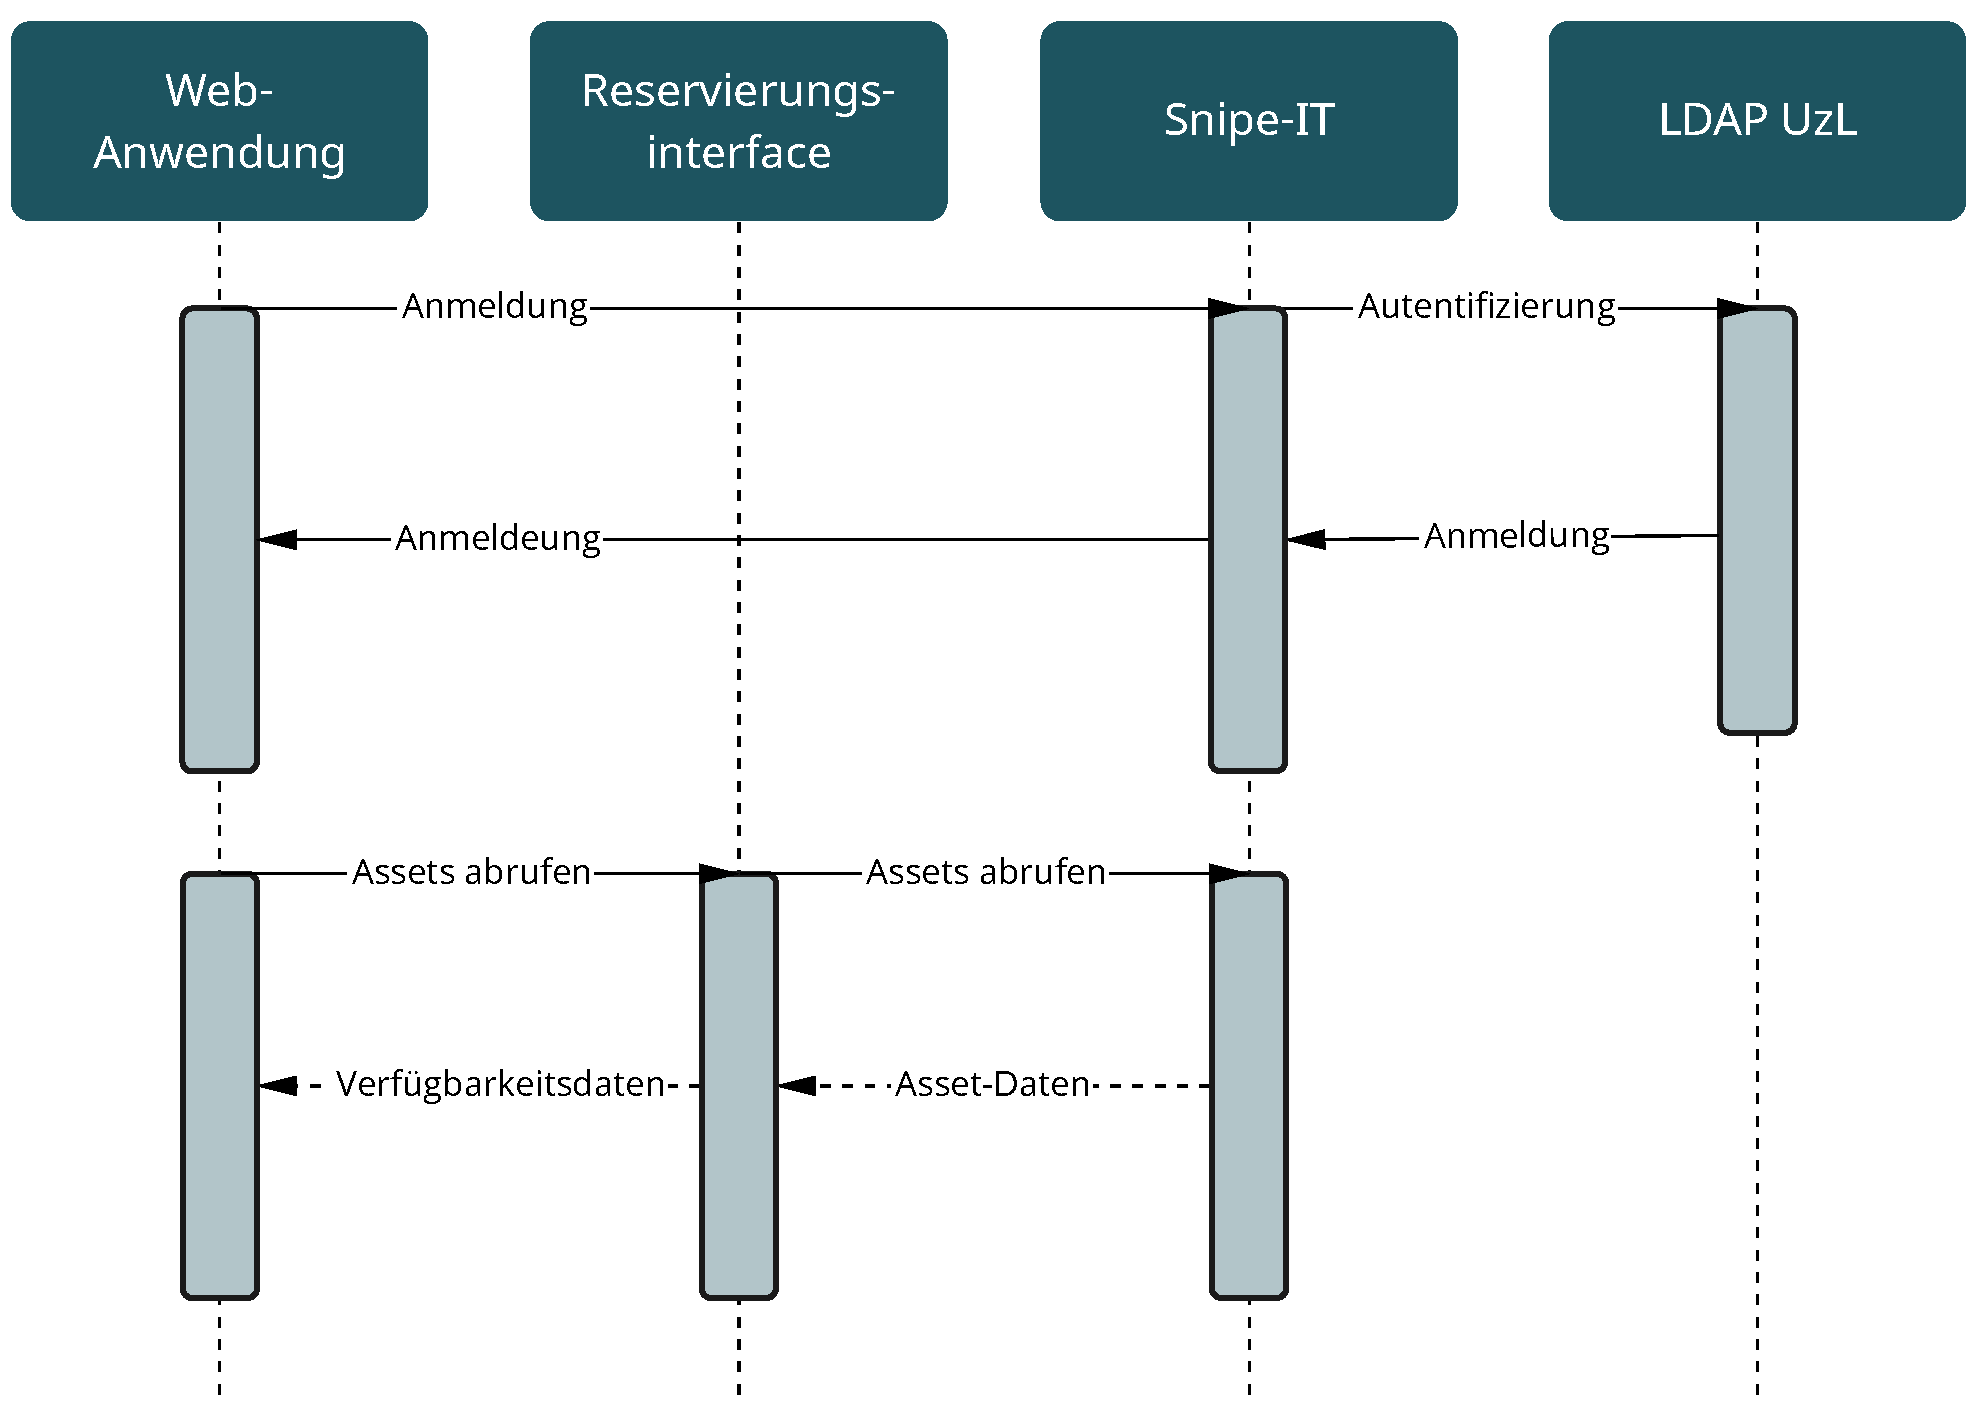
\includegraphics[scale=0.45]{Bilder/uml.pdf}
    \caption[UML-Sequenzdiagramm]{UML-Sequenzdiagramm}
    \label{fig:uml}
\end{figure}


